\documentclass[aspectratio=169]{beamer}

\usepackage{figures/tikzit}
\usepackage{graphicx}
\usepackage{etoolbox}
\usepackage{amssymb}
\usepackage{xparse}

\input{macros/sets}
\input{macros/category}
\input{macros/circuits}
\input{macros/streams}

\graphicspath{{./imgs/}}

\usetheme[
  background=light,
  numbering=counter,
  block=fill,
  %sectionpage=simple
]{metropolis}

\input{figures/circuits.tikzstyles}
\input{figures/circuits.tikzdefs}

% FiraFonts
\usepackage[sfdefault]{FiraSans}
\usepackage{FiraMono}
% Use thinner fonts
\makeatletter
\def\bfseries@sf{medium}
\def\mdseries@sf{l}
\makeatother

\newtoggle{static}
\settoggle{static}{false}

\definecolor{backg}{RGB}{9,72,61}
\definecolor{accent}{RGB}{0,150,136}

\definecolor{dracback}{RGB}{40, 42, 54}
\definecolor{dracfore}{RGB}{248, 248, 242}
\definecolor{dractitle}{RGB}{56, 58, 89}
\definecolor{dracblock}{RGB}{98, 114, 164}
\definecolor{draccent}{RGB}{255, 121, 198}

\setbeamercolor{normal text}{bg=dracfore}
\setbeamercolor{frametitle}{bg=dractitle, fg=dracfore}
\setbeamercolor{title separator}{fg=draccent}
\setbeamercolor{progress bar}{fg=draccent, bg=draccent}
\setbeamercolor{block title}{fg=dracfore, bg=dracblock}
\setbeamercolor{alerted text}{fg=draccent}

\newcommand{\wait}{\iftoggle{static}{}{\pause}}

\newtheorem{proposition}{Proposition}

\title{A compositional theory of digital circuits}
\author{
    \texorpdfstring{
        \large\textbf{George Kaye} \\[0.25em]
        \footnotesize University of Birmingham
    }{
        George Kaye
    }
}
\date{
    \texorpdfstring{
        07 February 2023 -- LFCS seminar, Edinburgh
    }{
        07 February 2023
    }
}

\begin{document}
    \maketitle
    % !TeX root = ../main.tex
\begin{frame}
    \frametitle{How we got here}
    \centering
    \wait
    \raisebox{-3em}{
        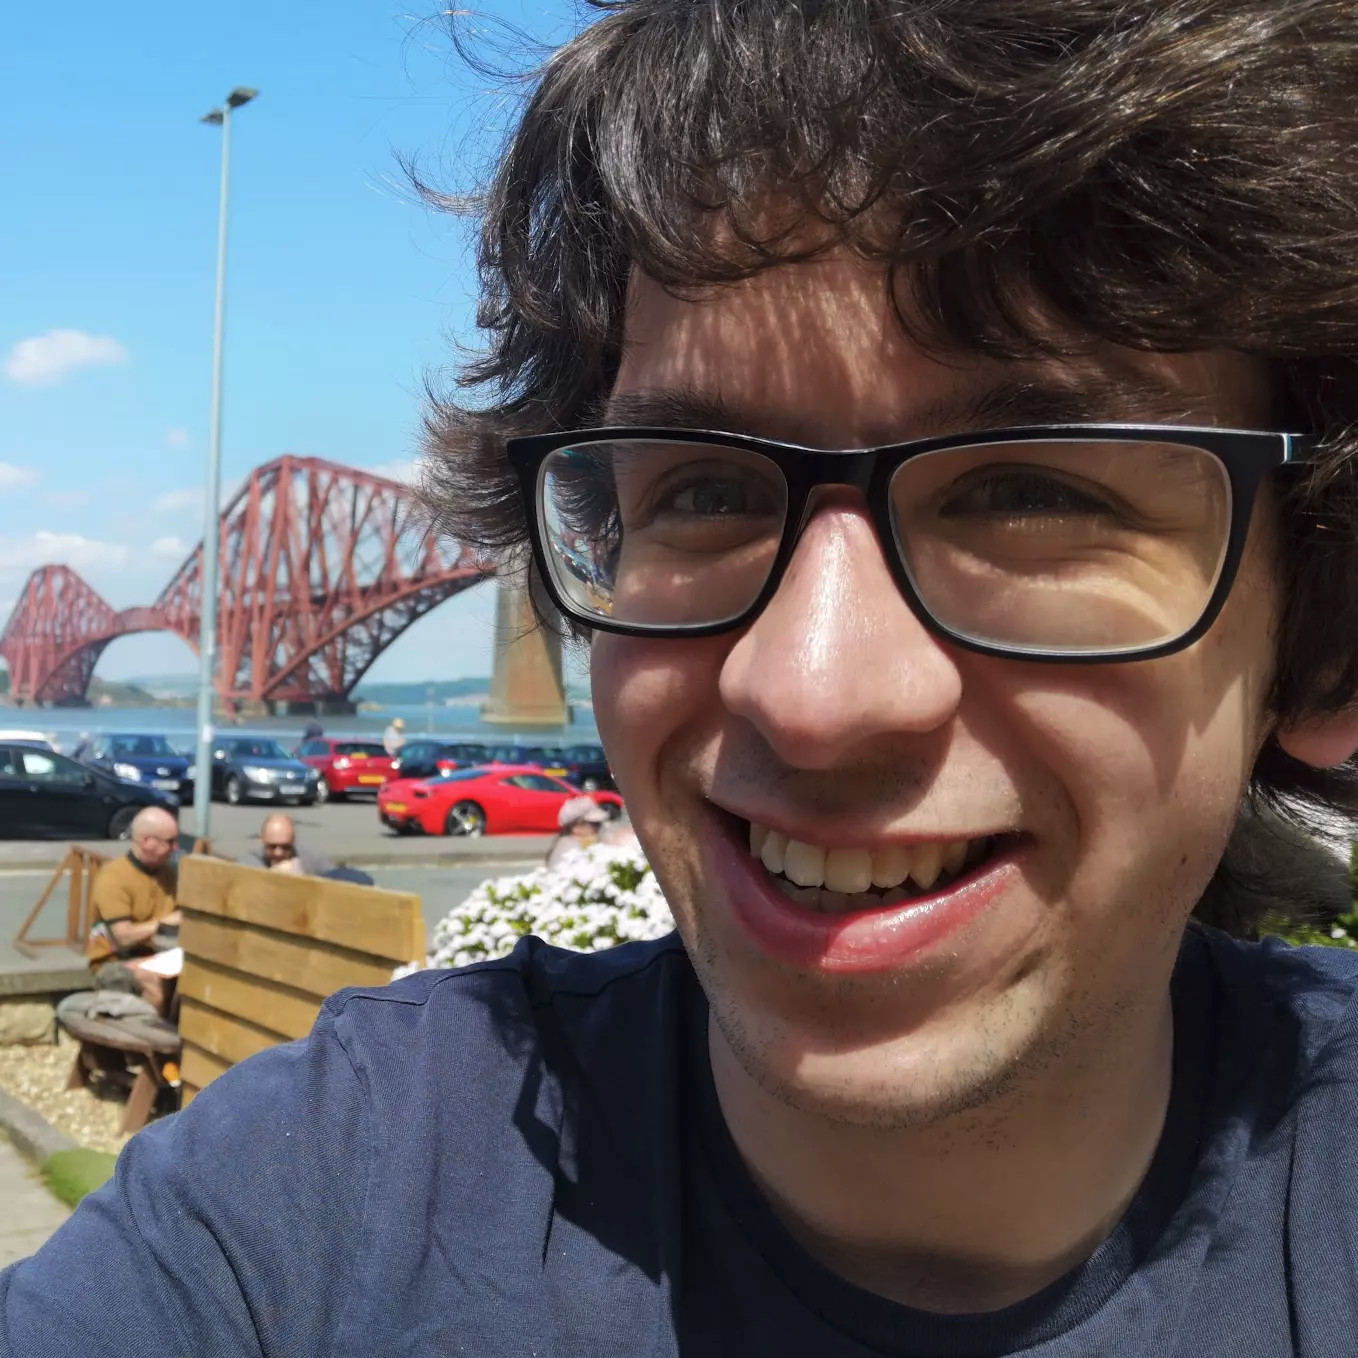
\includegraphics[width=0.2\textwidth]{imgs/me}
    }
    \qquad
    \begin{minipage}{0.7\textwidth}
        \emph{`Hi Ohad, want to do a seminar at Birmingham?'}
    \end{minipage}

    \wait
    \LARGE
    \textbf{Six months later...}
    \normalsize
    \wait

    \begin{minipage}{0.6\textwidth}
        \emph{`How about you do a seminar at Edinburgh first?'}
    \end{minipage}
    \qquad
    \raisebox{-3em}{
        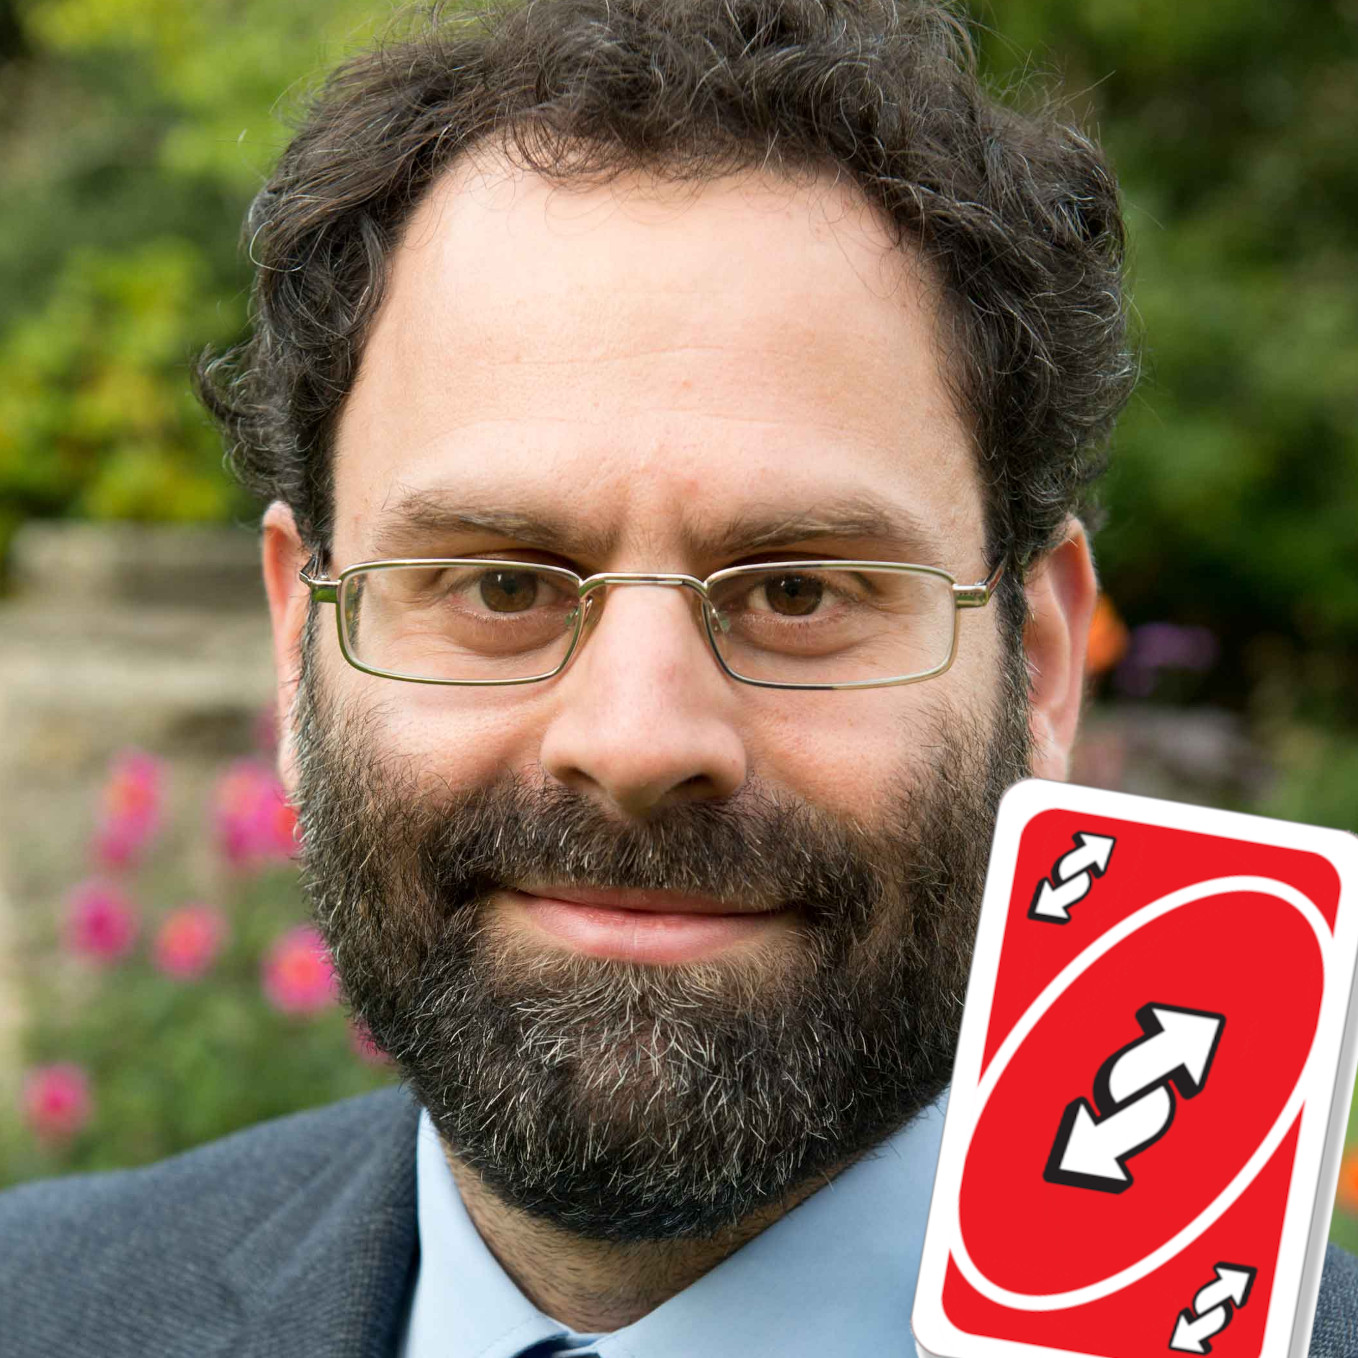
\includegraphics[width=0.2\textwidth]{imgs/ohad}
    }
\end{frame}

\begin{frame}
    \frametitle{What are we going to be talking about?}

    \centering
    \LARGE
    Digital circuits!

    \begin{center}
        \visible<2>{
            \only<-2>{
                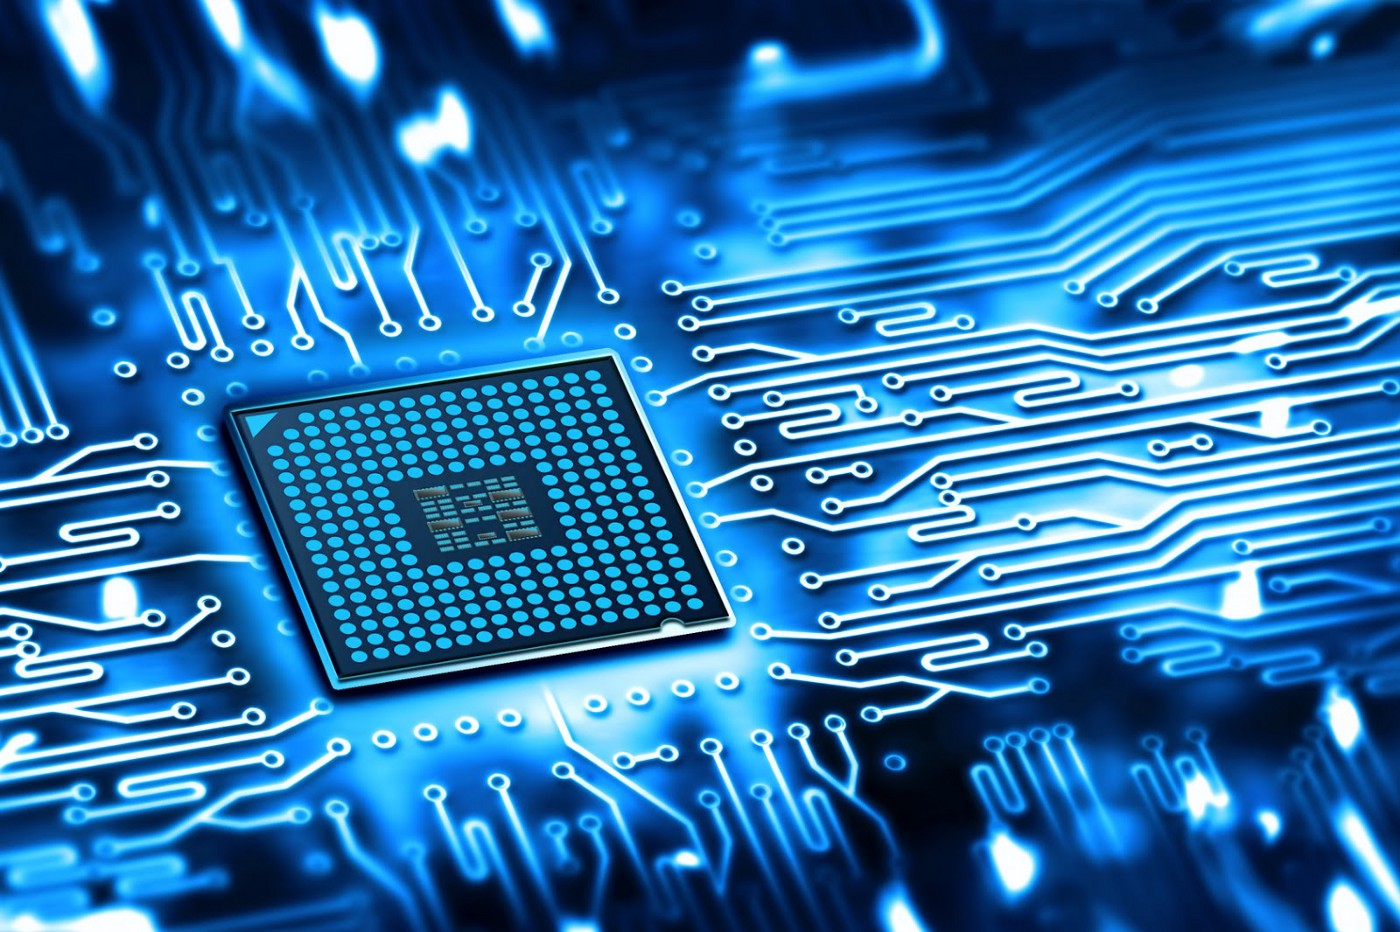
\includegraphics[width=0.6\textwidth]{imgs/circuit}
            }
        }
        \only<3>{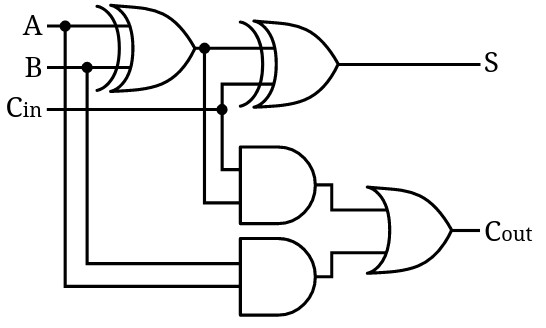
\includegraphics[width=0.6\textwidth]{imgs/adder}}
    \end{center}

\end{frame}

\begin{frame}
    \frametitle{What are we going to be talking about?}

    \centering
    \LARGE
    We want a \alert{compositional} theory of digital circuits.

    \vspace{0.5em}

    \dsptikzfig{strings/category/f-2-2}[F][seq]
    \dsptikzfig{strings/category/f-2-2}[G][seq]

    \vspace{0.5em}

    \dsptikzfig{strings/category/composition-2-2}[F][G][seq]
    \wait
    \quad
    \dsptikzfig{strings/monoidal/tensor-2-2}[F][G][seq]
    \wait
    \quad
    \dsptikzfig{strings/traced/trace-rhs}[F][seq]

    \wait
    \vspace{0.5em}

    These operations may look familiar to you!

\end{frame}

\begin{frame}
    \frametitle{Joint work with...}

    \begin{minipage}{0.49\textwidth}
        \centering
        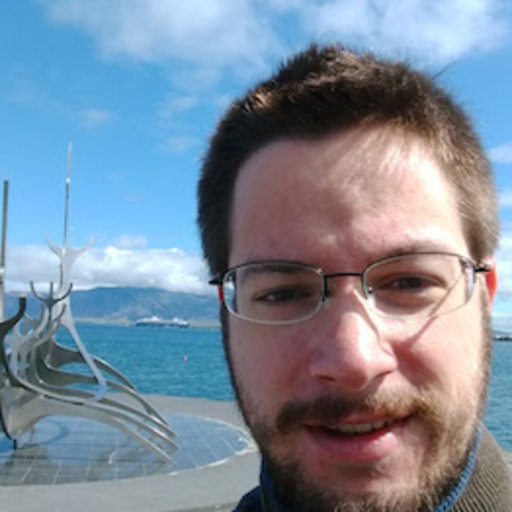
\includegraphics[width=0.5\textwidth]{imgs/sprunger}

        David Sprunger

        \scriptsize
        Indiana State University
    \end{minipage}
    \wait
    \begin{minipage}{0.49\textwidth}
        \centering
        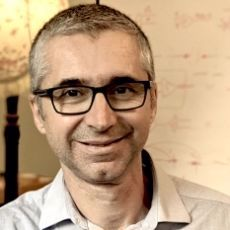
\includegraphics[width=0.5\textwidth]{imgs/ghica}

        Dan Ghica

        \scriptsize
        University of Birmingham
    \end{minipage}
\end{frame}
    \section{Syntax}

\begin{frame}
    \frametitle{Combinational circuit components}
    \renewcommand{\arraystretch}{1.25}
    \vspace{1em}
    \wait
    \begin{minipage}{0.33\textwidth}
        \centering
        \alert{gates}
        \renewcommand{\arraystretch}{2}

        \vspace{1em}

        \begin{tabular}{rl}
            \dsptikzfig{circuits/components/gates/and} &
            AND gate \\
            \dsptikzfig{circuits/components/gates/or} &
            OR gate \\
            \dsptikzfig{circuits/components/gates/not} &
            NOT gate \\
        \end{tabular}
    \end{minipage}
    \wait
    \begin{minipage}{0.32\textwidth}
        \centering
        \alert{(co)monoid structure}

        \vspace{1em}

        \renewcommand{\arraystretch}{1.75}
        \wait
        \begin{tabular}{cl}
            \hspace{0.175cm}
            \dsptikzfig{strings/structure/monoid/init}[comb] &
            disconnected \\
            \wait
            \dsptikzfig{strings/structure/comonoid/copy}[comb] &
            fork \\
            \wait
            \dsptikzfig{strings/structure/monoid/merge}[comb] &
            join \\
            \wait
            \dsptikzfig{strings/structure/comonoid/discard}[comb]
            \hspace{0.175cm} &
            stub \\
        \end{tabular}
    \end{minipage}
    \wait
    \begin{minipage}{0.32\textwidth}
        \centering
        \alert{categorical structure}

        \vspace{1em}

        \renewcommand{\arraystretch}{1.75}
        \begin{tabular}{cl}
            \wait
            \dsptikzfig{strings/category/identity}[comb] &
            identity \\
            \wait
            \dsptikzfig{strings/symmetric/symmetry}[comb] &
            symmetry \\
        \end{tabular}
    \end{minipage}


    \vspace{0.5em}

    \wait
    \begin{center}
        \alert{Light} circuits \(
            \dsptikzfig{strings/category/f}[F][comb]
        \) only contain gates and structure.
    \end{center}
\end{frame}
\begin{frame}
    \frametitle{Sequential circuit components}

    \wait

    \centering
    We need \alert{state}.

    \renewcommand{\arraystretch}{1.75}

    \wait

    \begin{minipage}{0.3\textwidth}
        \centering
        \alert{Values}

        \wait

        \begin{tabular}{rl}
            \dsptikzfig{circuits/components/values/v}[\belnapfalse] &
            false \\
            \dsptikzfig{circuits/components/values/v}[\belnaptrue] &
            true \\
            \wait
            \dsptikzfig{circuits/components/values/v}[\belnapboth] &
            short circuit
        \end{tabular}

        \vspace{1em}

        Along with \(
            \iltikzfig{strings/structure/monoid/init}[comb]
        \), models \emph{Belnap's four value logic}
    \end{minipage}
    \wait
    \begin{minipage}{0.3\textwidth}
        \centering
        \alert{Delay}

        \[
            \dsptikzfig{circuits/components/waveforms/delay}
        \]
    \end{minipage}
    \wait
    \begin{minipage}{0.3\textwidth}
        \centering
        \alert{Feedback}

        \[
            \dsptikzfig{strings/category/f-2-2}[F][seq]
            \,\,\Rightarrow\,\,
            \dsptikzfig{strings/traced/trace-rhs}[F][seq]
        \]
    \end{minipage}

    \vspace{1em}

    \wait

    \begin{center}
        \alert{Dark} circuits \(
            \dsptikzfig{strings/category/f}[F][seq]
        \) may contain delay or feedback.
    \end{center}
\end{frame}
\begin{frame}
    \frametitle{Building circuits}

    \centering
    \LARGE
    Circuits are morphisms in a
    \alert{freely generated symmetric traced monoidal category} (STMC).

    \wait
    \dsptikzfig{strings/category/composition-2-2}[F][G][seq]
    \wait
    \quad
    \dsptikzfig{strings/monoidal/tensor-2-2}[F][G][seq]
    \wait
    \quad
    \dsptikzfig{strings/traced/trace-rhs}[F][seq]

    \wait

    \vspace{1em}

    \Huge
    \(\scirc{}\)
\end{frame}

    \section{Semantics}

\begin{frame}
    \frametitle{We need some meaning}

    \wait
    Values are interpreted in a \alert{lattice}:
    \wait
    \begin{minipage}{0.49\textwidth}
        \[
            \scalebox{1.5}{\tikzfig{circuits/a4}}
        \]
    \end{minipage}
    \wait
    \begin{minipage}{0.49\textwidth}
        \begin{align*}
            \dsptikzfig{circuits/components/values/v}[\belnapfalse]
            \,&\mapsto\, 0 \\
            \dsptikzfig{circuits/components/values/v}[\belnaptrue]
            \,&\mapsto\, 1 \\
            \dsptikzfig{circuits/components/values/v}[\belnapboth]
            \,&\mapsto\, \top \\
            \dsptikzfig{strings/structure/monoid/init}[comb]
            \,&\mapsto\, \bot \\
        \end{align*}
    \end{minipage}
\end{frame}
\begin{frame}
    \frametitle{Let's make everything a function}

    \wait
    \setlength{\tabcolsep}{1.5em}
    \renewcommand{\arraystretch}{2}

    \begin{center}
        \begin{tabular}{lrl}
            \dsptikzfig{circuits/components/gates/gate}[g]
            &
            \alert{monotone functions}
            &
            \(\morph{\overline{g}}{\valuetuple{m}}{\values}\)
            \\
            \wait
            \hspace{0.175cm}
            \dsptikzfig{strings/structure/monoid/init}[comb]
            &
            \alert{initialise}
            &
            \(() \mapsto (\bot)\)
            \\
            \wait
            \dsptikzfig{strings/structure/comonoid/copy}[comb]
            &
            \alert{copy}
            &
            \(x \mapsto (x, x)\)
            \\
            \wait
            \dsptikzfig{strings/structure/monoid/merge}[comb]
            &
            \alert{join in the lattice}
            &
            \((x, y) \mapsto x \ljoin y\)
            \\
            \wait
            \dsptikzfig{strings/structure/comonoid/discard}[comb]
            &
            \alert{discard}
            &
            \(x \mapsto \bullet\)
        \end{tabular}
        \wait

        \vspace{0.5em}

        Feedback is interpreted as the \alert{least fixed point}.
    \end{center}
\end{frame}
\begin{frame}
        \frametitle{Functions are not enough}

        \centering
        \LARGE
        How do we model \alert{delay}?

        \wait
        \alert{Streams!}
\end{frame}
\begin{frame}
    \frametitle{Streams}

    A \alert{stream} \(\stream{\values}\) is an infinite sequence of values.
    \[
        v_0
        \streamcons
        v_1
        \streamcons
        v_2
        \streamcons
        v_3
        \streamcons
        v_4
        \streamcons
        v_5
        \streamcons
        v_6
        \streamcons
        v_7
        \streamcons
        \cdots
    \]

    \wait
    A \alert{stream function} \(\stream{\values} \to \stream{\values}\) consumes and
    produces streams.
    \[
        f(
            v_0
            \streamcons
            v_1
            \streamcons
            v_2
            \streamcons
            v_3
            \streamcons
            v_4
            \streamcons
            \cdots
        ) =
        w_0
        \streamcons
        w_1
        \streamcons
        w_2
        \streamcons
        w_3
        \streamcons
        w_4
        \streamcons
        \cdots
    \]
\end{frame}
\begin{frame}
    \frametitle{Interpreting the sequential components}
    \wait
    \[
        \dsptikzfig{circuits/components/values/v}[v]()
        :=
        v \streamcons \bot \streamcons \bot \streamcons \bot \streamcons \cdots
    \]

    \wait
    \vspace{1em}

    \[
        \dsptikzfig{circuits/components/waveforms/delay}(
            v_0 \streamcons v_1 \streamcons v_2 \streamcons \cdots
        )
        :=
        \bot \streamcons v_0 \streamcons v_1 \streamcons v_2 \streamcons \cdots
    \]
\end{frame}
\begin{frame}{Maybe there are too many streams}

    \centering
    \LARGE
    Does every circuit correspond to a stream function \(
        \valuetuplestream{m} \to \valuetuplestream{n}
    \)?

    \Huge
    \wait
    No.

    \scriptsize
    \wait
    (but this is to be expected!)
\end{frame}
\begin{frame}
    \frametitle{Circuits are causal and monotone}

    \wait
    \Large
    Circuits are \alert{causal}.

    \wait

    \normalsize
    They can only depend \alert{what they've seen so far}.

    \wait

    \Large
    Circuits are \alert{monotone}.

    \wait

    \normalsize
    They are constructed from \alert{monotone functions}.

    \wait

    Is that all?
    \wait
    \alert{Not quite...}
    \wait
    (but we'll get there)


\end{frame}
\begin{frame}
    \frametitle{Some operations on stream function}

    Given a causal stream function \(
        \morph{f}{\valuetuplestream{m}}{\valuetuplestream{n}}
    \) and an element \(a \in \valuetuple{m}\)...

    \wait

    \Large
    \alert{initial output} \quad
    \(\mealyoutput{f}{a} \in \valuetuple{n}\)

    \wait

    \normalsize
    `the first thing \(f\) produces given \(a\)'

    \wait

    \Large
    \alert{stream derivative} \quad
    \(\mealytransition{f}{a} \in \valuetuplestream{m} \to \valuetuplestream{n}\)

    \wait

    \normalsize
    `how \(f\) behaves after seeing \(a\) first'

    \vspace{1em}

    \wait
    Hold on, these look familiar...

\end{frame}
\begin{frame}
    \frametitle{An old friend}

    \Large

    \begin{center}
        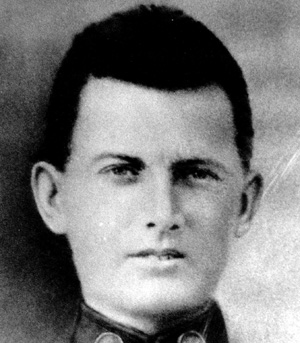
\includegraphics[width=0.3\textwidth]{imgs/mealy}
        \quad
        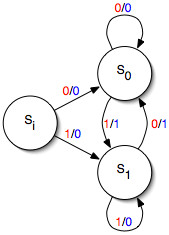
\includegraphics[scale=0.5]{imgs/mealy-machine}

        Mealy machine moment!

        \wait

        \normalsize
        Stream functions are the \emph{states} in a Mealy machine.
    \end{center}

\end{frame}
\begin{frame}
    \frametitle{Circuits have finitely many behaviours}

    Circuits have a finite number of components.

    \wait

    So there are finite number of states in the Mealy machine.

    \wait

    So the outputs of streams given some input must be \alert{periodic}.

    \wait

    (There are finitely many \alert{stream derivatives}).
\end{frame}
\begin{frame}
    \frametitle{These are the streams we're looking for}

    \begin{theorem}
        A stream function is the interpretation of a sequential circuit
        if and only if it is \textbf{causal}, \textbf{monotone} and has
        \textbf{finitely many stream derivatives}.
    \end{theorem}
\end{frame}
    \section{Equational reasoning}

\begin{frame}
    \frametitle{Now what?}

    We have a \alert{sound and complete} semantics for circuits as
    \alert{stream functions}.

    \wait

    But reasoning with streams can be a \alert{pain}...

    \wait
    Why not reason \alert{equationally}?
\end{frame}
\begin{frame}
    \frametitle{The two types of equation}

    \centering
    \begin{minipage}{0.49\textwidth}
        \centering
        \alert{Global}

        \vspace{1.5em}

        \dsptikzfig{strings/structure/cartesian/naturality-copy-lhs}[F][seq]
        =
        \dsptikzfig{strings/structure/cartesian/naturality-copy-rhs}[F][seq]
    \end{minipage}
    \begin{minipage}{0.49\textwidth}
        \centering
        \alert{Local}

        \vspace{1.5em}

        \dsptikzfig{circuits/axioms/fork-lhs}[v]
        =
        \dsptikzfig{circuits/axioms/fork-rhs}[v]
    \end{minipage}

    \vspace{1.5em}

    We want to stick to local equations \alert{as much as possible}.

\end{frame}

\begin{frame}
    \frametitle{What do the values do?}

    \centering
    \begin{axiom}
        \begin{minipage}{0.32\textwidth}
            \begin{equation*}
                \dsptikzfig{circuits/axioms/gate-lhs}
                =
                \dsptikzfig{circuits/axioms/gate-rhs-simple}
            \end{equation*}

            \visible<3->{
                \begin{equation*}
                    \dsptikzfig{circuits/axioms/join-lhs}[v][w]
                    =
                    \dsptikzfig{circuits/axioms/join-rhs}[v][w]
                \end{equation*}
            }
        \end{minipage}
        \begin{minipage}{0.32\textwidth}
            \visible<2->{
                \begin{equation*}
                    \dsptikzfig{circuits/axioms/fork-lhs}[v]
                    =
                    \dsptikzfig{circuits/axioms/fork-rhs}[v]
                \end{equation*}
            }

            \visible<4->{
                \begin{equation*}
                    \dsptikzfig{circuits/axioms/stub-lhs}[v]
                    =
                    \dsptikzfig{strings/monoidal/empty}
                \end{equation*}
            }
        \end{minipage}
        \begin{minipage}{0.32\textwidth}
            \visible<5->{
                \begin{equation*}
                    \dsptikzfig{circuits/axioms/disconnect-lhs}
                    =
                    \dsptikzfig{circuits/axioms/disconnect-rhs}
                \end{equation*}
            }
        \end{minipage}
    \end{axiom}

    \wait

    \visible<6->{
        For \(
            \dsptikzfig{circuits/components/values/v}[\overline{v}]
        \) and \(
            \dsptikzfig{strings/category/f}[F][comb]
        \), there exists \(
            \dsptikzfig{circuits/components/values/v}[\overline{w}]
        \) such that \(
            \dsptikzfig{circuits/components/circuits/f-applied}[F][comb][\overline{v}]
            =
            \dsptikzfig{circuits/components/values/v}[\overline{w}]
        \).
    }
\end{frame}
\begin{frame}
    \frametitle{Let's get structural}

    \centering
    \wait

    \((
        \dsptikzfig{strings/structure/monoid/merge}[comb],
        \dsptikzfig{strings/structure/monoid/init}[comb],
        \dsptikzfig{strings/structure/comonoid/copy}[comb],
        \dsptikzfig{strings/structure/comonoid/discard}[comb],
    )\) is a \alert{bialgebra}.
    \wait
    \begin{axiom}
        \centering
        \begin{minipage}{0.21\textwidth}
            \begin{equation*}
                \dsptikzfig{strings/structure/monoid/unitality-l-lhs}
                =
                \dsptikzfig{strings/structure/monoid/unitality-l-rhs}
            \end{equation*}
        \end{minipage}
        \quad
        \begin{minipage}{0.26\textwidth}
            \begin{equation*}
                \dsptikzfig{strings/structure/monoid/associativity-lhs}
                =
                \dsptikzfig{strings/structure/monoid/associativity-rhs}
            \end{equation*}
        \end{minipage}
        \quad
        \begin{minipage}{0.26\textwidth}
            \begin{equation*}
                \dsptikzfig{strings/structure/monoid/commutativity-lhs}
                =
                \dsptikzfig{strings/structure/monoid/commutativity-rhs}
            \end{equation*}
        \end{minipage}

        \begin{minipage}{0.21\textwidth}
            \begin{equation*}
                \dsptikzfig{strings/structure/comonoid/unitality-l-lhs}
                =
                \dsptikzfig{strings/structure/comonoid/unitality-l-rhs}
            \end{equation*}
        \end{minipage}
        \quad
        \begin{minipage}{0.26\textwidth}
            \begin{equation*}
                \dsptikzfig{strings/structure/comonoid/associativity-lhs}
                =
                \dsptikzfig{strings/structure/comonoid/associativity-rhs}
            \end{equation*}
        \end{minipage}
        \quad
        \begin{minipage}{0.26\textwidth}
            \begin{equation*}
                \dsptikzfig{strings/structure/comonoid/commutativity-lhs}
                =
                \dsptikzfig{strings/structure/comonoid/commutativity-rhs}
            \end{equation*}
        \end{minipage}

        \begin{minipage}{0.28\textwidth}
            \begin{equation*}
                \dsptikzfig{strings/structure/bialgebra/merge-copy-lhs}
                =
                \dsptikzfig{strings/structure/bialgebra/merge-copy-rhs}
            \end{equation*}
        \end{minipage}
        \begin{minipage}{0.23\textwidth}
            \begin{equation*}
                \dsptikzfig{strings/structure/bialgebra/init-copy-lhs}
                =
                \dsptikzfig{strings/structure/bialgebra/init-copy-rhs}
            \end{equation*}
        \end{minipage}
        \begin{minipage}{0.23\textwidth}
            \begin{equation*}
                \dsptikzfig{strings/structure/bialgebra/merge-discard-lhs}
                =
                \dsptikzfig{strings/structure/bialgebra/merge-discard-rhs}
            \end{equation*}
        \end{minipage}
        \begin{minipage}{0.2\textwidth}
            \begin{equation*}
                \dsptikzfig{strings/structure/bialgebra/init-discard-lhs}
                =
                \dsptikzfig{strings/structure/bialgebra/init-discard-rhs}
            \end{equation*}
        \end{minipage}
    \end{axiom}
\end{frame}
\begin{frame}
    \frametitle{Splitting things up}

    \centering

    \alert{Isolate} the sequential and combinational components...

    \wait
    \[
        \dsptikzfig{strings/category/f}[F][seq]
        =
        \dsptikzfig{circuits/productivity/pre-mealy-form-verbose}[F][s]
    \]

    \wait
    This is \emph{almost} another Mealy machine moment...
    \raisebox{-1.5em}{
        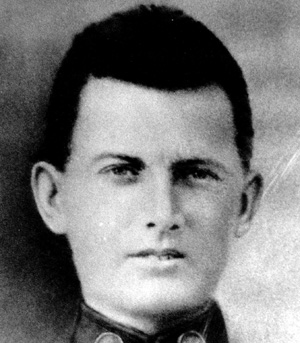
\includegraphics[width=0.1\textwidth]{imgs/mealy}
    }

    \wait
    ...but there is the non-delay-guarded trace!
\end{frame}
\begin{frame}
    \frametitle{Do we even need it?}

    In industry, normally circuits must be \alert{delay-guarded}.

    \wait

    But this rules out some \alert{clever} circuits!

    \vspace{0.5em}

    \scalebox{0.75}{
        \dsptikzfig{circuits/examples/cyclic-combinational/circuit-scirc}
        \(\Rightarrow\)
        \dsptikzfig{circuits/examples/cyclic-combinational/reduced-true}
    }

    \wait

    \vspace{0.5em}

    \scriptsize
    (And also it would be cheating)

\end{frame}
\begin{frame}
    \frametitle{Getting rid of non-delay-guarded feedback}

    \(\values\) is a \alert{finite} lattice...\

    \wait
    The functions are monotone...

    \wait
    We can compute the \alert{least fixed point} in finite iterations!
    \wait

    \centering
    \[
        \dsptikzfig{circuits/instant-feedback/f0-box}
        :=
        \dsptikzfig{circuits/instant-feedback/f0-definition}
        \wait
        \qquad
        \dsptikzfig{circuits/instant-feedback/fkp1-box}
        :=
        \dsptikzfig{circuits/instant-feedback/fkp1-definition}
    \]

    \begin{axiom}
        \[
            \dsptikzfig{circuits/instant-feedback/equation-lhs}[F][][][x]
            \quad
            =
            \quad
            \dsptikzfig{circuits/instant-feedback/fixpoint-concrete}
        \]
    \end{axiom}
\end{frame}
\begin{frame}
    \frametitle{Getting rid of non-delay-guarded feedback}


    \[
        \dsptikzfig{circuits/instant-feedback/trand}
        \quad
        \wait
        =
        \quad
        \dsptikzfig{circuits/instant-feedback/trand-instfb}
        =
        \wait
        \quad
        \dsptikzfig{strings/structure/monoid/init}[comb]
    \]


\end{frame}
\begin{frame}
    \frametitle{Here's Mealy}

    \centering
    For \alert{any} circuit

    \[
        \dsptikzfig{strings/category/f}[F][seq]
        \quad
        =
        \quad
        \dsptikzfig{circuits/productivity/mealy-form-verbose}[F][\overline{s}]
    \]
    
    \wait

    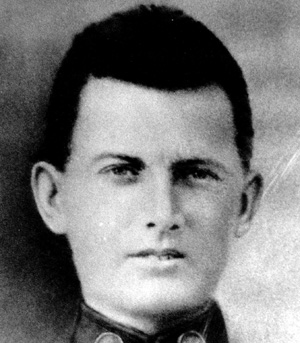
\includegraphics[width=0.25\textwidth]{imgs/mealy}

\end{frame}
\begin{frame}
    \frametitle{Let's get (even more) structural}

    What more structure can we add?

    \wait

    \alert{Forking} is natural...

    \wait

    \begin{axiom}
        \begin{minipage}{0.33\textwidth}
            \begin{equation*}
                \dsptikzfig{circuits/axioms/fork-gate-lhs}
                =
                \dsptikzfig{circuits/axioms/fork-gate-rhs}
            \end{equation*}
        \end{minipage}
        \begin{minipage}{0.33\textwidth}
            \begin{equation*}
                \dsptikzfig{circuits/axioms/fork-delay-lhs}
                =
                \dsptikzfig{circuits/axioms/fork-delay-rhs}
            \end{equation*}
        \end{minipage}
    \end{axiom}

    For any circuit...
    \(
        \dsptikzfig{strings/structure/cartesian/naturality-copy-lhs}[F][seq]
        =
        \dsptikzfig{strings/structure/cartesian/naturality-copy-rhs}[F][seq]
    \)
\end{frame}
\begin{frame}
    \frametitle{Let's (even even more) structural}

    Let's do the same for \alert{stubbing}...

    \begin{axiom}
        \begin{minipage}{0.22\textwidth}
            \begin{equation*}
                \dsptikzfig{circuits/axioms/stub-gate-lhs}
                =
                \dsptikzfig{circuits/axioms/stub-gate-rhs}
            \end{equation*}
        \end{minipage}
        \wait
        \begin{minipage}{0.2\textwidth}
            \begin{equation*}
                \dsptikzfig{circuits/axioms/unobservable-lhs}
                =
                \dsptikzfig{circuits/axioms/unobservable-rhs}
            \end{equation*}
        \end{minipage}
        \wait
        \quad
        \begin{minipage}{0.3\textwidth}
            \begin{equation*}
                \dsptikzfig{circuits/axioms/delay-discard-lhs}[F]
                =
                \dsptikzfig{circuits/axioms/delay-discard-rhs}
            \end{equation*}
        \end{minipage}
    \end{axiom}

    For any circuit...
    \(
        \dsptikzfig{strings/structure/cartesian/naturality-discard-lhs}[F][seq]
        =
        \dsptikzfig{strings/structure/cartesian/naturality-discard-rhs}
    \)

\end{frame}
\begin{frame}
    \frametitle{Let's get structural}

    \centering
    \[
        \dsptikzfig{strings/structure/cartesian/naturality-copy-lhs}[F][seq]
        =
        \dsptikzfig{strings/structure/cartesian/naturality-copy-rhs}[F][seq]
        \qquad
        \dsptikzfig{strings/structure/cartesian/naturality-discard-lhs}[F][seq]
        =
        \dsptikzfig{strings/structure/cartesian/naturality-discard-rhs}
    \]

    \LARGE
    \wait
    Cartesian!
    \normalsize
    \wait
    \[
        \dsptikzfig{strings/traced/trace-rhs}[F][seq]
        =
        \dsptikzfig{circuits/examples/reasoning/unfolding/unfolding-3}[F][seq]
    \]


\end{frame}
\begin{frame}
    \frametitle{Running the simulation}

    \centering

    \LARGE
    Goal:
    \normalsize

    \begin{equation*}
        \dsptikzfig{circuits/productivity/productive-goal-lhs-verbose}[F][v]
        =
        \dsptikzfig{circuits/productivity/productive-goal-rhs-verbose}[G][w]
    \end{equation*}

\end{frame}
\begin{frame}
    \frametitle{Running the simulation}

    \begin{axiom}
        \wait
        \[
            \dsptikzfig{circuits/axioms/streaming-lhs-verbose}[g][v]
            =
            \dsptikzfig{circuits/axioms/streaming-rhs}[g][v]
            \wait
            \qquad
            \dsptikzfig{circuits/axioms/join-delay-lhs}
            =
            \dsptikzfig{circuits/axioms/join-delay-rhs}
        \]
    \end{axiom}

    \[
        \dsptikzfig{circuits/axioms/generalised-streaming-lhs-verbose}[F][v]
        =
        \dsptikzfig{circuits/axioms/generalised-streaming-rhs}[F][v]
        =
        \dsptikzfig{circuits/axioms/generalised-streaming-rhs-reduced}[F][v]
    \]

\end{frame}
\begin{frame}
    \frametitle{Running the simulation}
    \[
        \dsptikzfig{circuits/productivity/productive-goal-lhs-verbose}[F][v]
        \wait
        =
        \dsptikzfig{circuits/productivity/productive-lhs-verbose}[F][v][s]
    \]

    \vspace{0.5em}
    \wait
    \(
        = \dsptikzfig{circuits/productivity/productive-step-9}[F][s][v]
    \)
    \wait
    \raisebox{-3em}{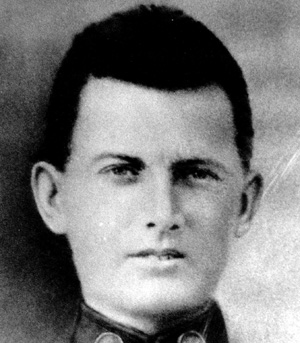
\includegraphics[width=0.2\textwidth]{imgs/mealy}}
\end{frame}

\end{document}